%!TEX program = xelatex
\documentclass[11pt,punct,twoside]{ctexart}
\usepackage{titling}
\usepackage[a4paper, left=3cm, right=2cm, top=3cm, bottom=2.5cm]{geometry}
\usepackage{fancyhdr, graphicx, xpatch, layout}
\usepackage{booktabs}
\usepackage{amsmath}
\usepackage{pdfpages}
\usepackage{float}
%\usepackage{cite}
\usepackage{enumitem}
\usepackage{titlesec}
\usepackage{titletoc}
\usepackage{tabularx}
\usepackage{chngcntr}
\usepackage{listings}
\usepackage{hyperref}
\usepackage{cleveref}
\usepackage{subfigure}
\usepackage[titles,subfigure]{tocloft}
\usepackage[labelsep=space]{caption}
\usepackage[numbers,super,square,comma,sort,compress]{natbib}
\usepackage{lmodern}
\usepackage{indentfirst}
\usepackage{xtab,booktabs}
\usepackage[version=4]{mhchem}
\usepackage{array}
\usepackage{fontspec}
\usepackage{caption}
\usepackage{xeCJK}
\usepackage{color}
\usepackage{longtable}
\usepackage{ctex}
%\usepackage{longtabu}
\usepackage{tabu}
\usepackage{makecell}
\usepackage{amssymb}
%\usepackage{showframe}
\usepackage{lastpage}

% 导入包

% 格式设置
\hypersetup{hidelinks,
	colorlinks=true,
	allcolors=black,
	pdfstartview=Fit,
	breaklinks=true}

% 微分算子
\newcommand*{\dif}{\mathop{}\!\mathrm{d}}

% 参考文献行间距
\setlength{\bibsep}{-1pt}
%设置字体
\setmainfont{Times New Roman} % set all eng font
\songti%正文宋体
\zihao{-4}%正文小四号
\ctexset{section={format+={\mdseries\zihao{3}\heiti},aftername = \hspace{0.5em}}}%章标题 三号黑体
\ctexset{subsection={format+={\mdseries\zihao{-4}\heiti},aftername = \hspace{0.5em}}}%节标题 小四号黑体
\ctexset{subsubsection={format+={\mdseries\zihao{-4}\heiti},aftername = \hspace{0.5em}}}%级标题 小四号黑体  

%宋体伪粗体
\setCJKfamilyfont{zhsong}[AutoFakeBold = {2.17}]{SimSun}
\renewcommand*{\songti}{\CJKfamily{zhsong}}
%设置间距
\renewcommand{\baselinestretch}{1.62}
%\linespread{1.5}
\titlespacing{\section}{0bp}{0.5em}{0.5em}
\titlespacing{\subsection}{0bp}{0.5em}{0.5em}
\titlespacing{\subsubsection}{0bp}{0.5em}{0.5em}
%\setlength{\parskip}{0.5\baselineskip}
% 图表公式每章重新编号
\counterwithin{table}{section}
\counterwithin{figure}{section}
\counterwithin{equation}{section}

%表标题与内容间距
\setlength{\abovecaptionskip}{0.1cm}
%列表样式
\setlist[enumerate,1]{label=(\arabic*), wide, labelsep=0.5em, itemsep=0ex, topsep=0pt, partopsep=0pt, parsep=0pt}
\setlist[enumerate,2]{label=(\alph*) , wide, labelsep=0.5em, itemsep=0ex, topsep=0pt, partopsep=0pt, parsep=0pt,itemindent=5em}

%正文代码块lstlisting样式
\def\inline{\lstinline[basicstyle=\ttfamily,breaklines=true]}
\lstset{
	basicstyle=\ttfamily\zihao{5},
	xleftmargin=2em,
	%xrightmargin=2em,
    breaklines=true,
    frame={tb},
    belowcaptionskip=0.6em,
    framerule=1.5pt
}

%引用样式
\renewcommand{\lstlistingname}{代码清单}
\crefname{listing}{代码清单}{代码清单}
\crefname{table}{表}{表}
\Crefname{table}{表}{表}
\crefname{figure}{图}{图}
\Crefname{figure}{图}{图}

%自定义命令
\newcommand{\scite}[1]{\textsuperscript{\cite{#1}}} %cite样式
\DeclareCaptionFormat{myformat}{\zihao{5}\selectfont#1#2#3}
\captionsetup{format=myformat}
\captionsetup{labelsep=quad}%图表号与图表名之间空两格

%------------------文档开始------------------
\begin{document}
\pagestyle{plain}
\lfoot{}
\cfoot{\zihao{5}\thepage}
\rfoot{}
\pagenumbering{Roman} %目录页码为罗马数字
	\begin{center}
		\heiti \zihao{3} 2022年首届“钉钉杯”大学生大数据挑战赛论文
		
		\section*{\zihao{-3}\heiti 基于XGB、LGB、随机森林的Stacking诈骗预测模型}
		\section*{\zihao{3}\heiti 摘\ \ \ \ \ \ \ \ 要}
	\end{center}


随着互联网的迅猛发展以及移动支付的普及,银行卡电信诈骗的问题愈加严峻。本文通对银行卡交易信息数据进行EDA、特征工程、建立模型、模型调参、模型融合、模型评价,建立了基于XGB、LGB、随机森林的Stacking诈骗预测模型,最终选择Stackin作为预测模型,模型准确率为0.9999987,F-1值为0.999885。最后给客户提出建议\textbf{:用户如果能够使用pin交易,那么将会使欺诈发生的概率趋近于0;当用户发现当前交易是往期交易的数倍时,用户需要谨慎思考当前是否遭遇了银行卡欺诈行为}。从Kaggle获取我们的代码:\href{github首页}{https://www.kaggle.com/code/zhouhua2022/card-transdata}

\textbf{EDA}:导入需要用到的包,读取数据;查看数据基本信息,查看7个分类属性数据的分布情况,查看标签在7个分类属性条件下的分布情况。


\textbf{数据预处理}:第一步,对数据进行\textbf{异常值处理}。查看3个连续型属性的分布,发现只有极少的值是异常值,考虑到异常数值对应属性在实际生活中是切实存在的,并且异常值处理前后平均值与方差的变化在5\%以内,因此不对数据进行异常值处理。第二步,对三个连续型属性数据进行\textbf{标准化}。第三步,对4个分类属性数据进行\textbf{独热编码}。第四步,\textbf{选择分类特征}。查看属性的相关系数矩阵,发现属性间相关性小,属性独立性好,故没有进一步对数据降维的必要。第五步,\textbf{数据集划分}。对数据集进行划分,训练集与测试集比例为7:3。

\textbf{模型建立}:使用LGB,XGB,KNN,线性SVC,朴素贝叶斯,决策树随机森林,感知机,逻辑回归,随机剃度下降\textbf{10个模型}对数据进行拟合并查看在测试集上的准确率,其中决策树,随机森林的准确率达到了\textbf{100\%}


\textbf{模型调参与模型融合}:第一步,\textbf{模型调参}。选取XGB、LGB、KNN、决策树、随机森林5个准确度最高的模型,使用网格搜索调节参数。第二步,\textbf{模型融合}。从调节参数之后的5个模型中选出三个表现最好的XGB、LGB、随机森林建立Stacking模型。



\textbf{模型评价与可视化}:计算6个模型的$precision$、$recall$、$f1-score$,画出6个模型的混淆矩阵热力图、ROC曲线,最后根据F1分数值选出最优模型为Stacking模型。


\textbf{提出建议}:通过标签与分类属性的数据分布情况、标签与分类属性的相关性系数、决策树特征重要性分析,给客户提出合理建议。



\par


\par
%空一行

\noindent \zihao{-4}{\heiti 关键词:}\textbf{XGB};\textbf{随机森林};\textbf{Stacking模型};\textbf{F1分数值}

\clearpage



%目录样式
% \renewcommand{\cftdot}{\ensuremath{\ast}}
\titlecontents{section}
[1em]
{\heiti\zihao{-4}}%
{\contentslabel{1em}}%
{}%
{\titlerule*[0.32pc]{$\cdot$}\contentspage}
\titlecontents{subsection}
[3.5em]
{\songti\zihao{-4}}%
{\contentslabel{1.7em}}%
{}%
{\titlerule*[0.32pc]{$\cdot$}\contentspage}
\titlecontents{subsubsection}
[6em]
{\songti\zihao{-4}}%
{\contentslabel{2.5em}}%
{}%
{\titlerule*[0.32pc]{$\cdot$}\contentspage}
\titlecontents{section*}
[0em]
{\heiti\zihao{-4}}%
{\contentslabel{1em}}%
{}%
{\titlerule*[0.32pc]{$\cdot$}\contentspage}
\renewcommand{\cftsecleader}{\cftdotfill{\cftdotsep}}
\newcommand\mydot[1]{\scalebox{#1}{.}}
\renewcommand\cftdot{\mydot{0.8}}
\renewcommand\cftdotsep{1}

%\captionsetup[contentsname={\zihao{3}目\ \ \ \ \ \ \ \ 录}]
\renewcommand{\contentsname}{\zihao{3}目\ \ \ \ \ \ \ \ 录}
\renewcommand{\cftsecfont}{\heiti\zihao{-4}} %设置section条目的字体
\renewcommand{\cftsecfont}{\heiti} %设置section条目的字体
%\renewcommand{\cftsecpagefont}{\normalfont}
\renewcommand{\cftsubsecfont}{\songti\zihao{-4}} %设置subsection条目的字体
\rhead{}
\tableofcontents
%\include{sections/statement}

\setlength{\voffset}{-10mm}                        
\setlength{\topmargin}{0mm}
\setlength{\headheight}{6mm}
\setlength{\headsep}{9mm}
\setlength{\footskip}{7.5mm}


%正文代码块章节编号
\counterwithin{lstlisting}{section}

%\include{sections/abstract}
%\include{sections/toc}
\pagenumbering{arabic} %正文页码为阿拉伯数字
%页眉页脚
\pagestyle{fancy}
\setcounter{page}{1}%页码重新计数
%\setlength{\voffset}{3pt}
\lhead{\zihao{4}\heiti Team ~ \# ~  2022071312193}
\chead{}
\rhead{\zihao{4}\heiti Page ~ \thepage ~ of ~ \pageref{LastPage}}

\section{绪论}
\subsection{研究背景}
随着互联网的迅猛发展以及移动支付的普及,多账户注册与支付方式变多导致用户信息泄露的情况越来越多,信息泄露导致银行卡交易欺诈行为增多。因此,根据用户交易信息对欺诈行为具有重要的意思。

数据集文件$“card\_transdata.csv”$中包含了100万条用户银行卡交易的信息,其中包括7个特征和一列标签,7个特征包含了用户交易时离家距离,交易数额变化,交易方式等信息,标签指出该笔交易是否存在欺诈行为。本文就是对银行卡交易信息进行分析,提取有效信息,建立模型,从而实现对欺诈行为的检测并对用户提出合理的建议从而减少欺诈行为的发生。



\subsection{研究思路}
\textbf{第一步(EDA)}:导入需要用到的包,读取数据;查看数据基本信息,查看7个分类属性数据的分布情况,查看标签在7个分类属性条件下的分布情况。


\textbf{第二步(数据预处理)}:首先对数据进行\textbf{异常值处理},通过查看3个连续型属性的分布,发现只有极少的值是异常值,考虑到异常数值对应属性在实际生活中是切实存在的,并且异常值处理前后平均值与方差的变化在5\%以内,因此不对数据进行异常值处理。然后对三个连续型属性数据进行\textbf{标准化}。紧接着对4个分类属性数据进行独热编码。之后选择分类特征,通过查看属性的相关系数矩阵,发现属性间相关性小,属性独立性好,故没有进一步对数据降维的必要。最后对数据集按7:3进行划分。

\textbf{第三步(模型建立)}:使用LGB,XGB,KNN,线性SVC,朴素贝叶斯,决策树随机森林,感知机,逻辑回归,随机剃度下降10个模型对数据进行拟合并查看在测试集上的准确率。


\textbf{第四步(模型调参与模型融合)}:首先进行模型调参,选取XGB、LGB、KNN、决策树、随机森林5个准确度最高的模型,使用网格搜索调节参数。然后进行模型融合,使用调节参数之后的5个模型建立Stacking模型。



\textbf{第五步(模型评价与可视化)}:计算6个模型的$precision$、$recall$、$f1-score$,画出6个模型的混淆矩阵热力图、ROC曲线,最后根据F1分数值选出最优模型为Stacking模型。


\textbf{第六步(提出建议)}:通过标签与分类属性的数据分布情况、标签与分类属性的相关性系数、决策树特征重要性分析,给客户提出合理建议。


具体研究思路如下:
\begin{figure}[H]
	\centering
	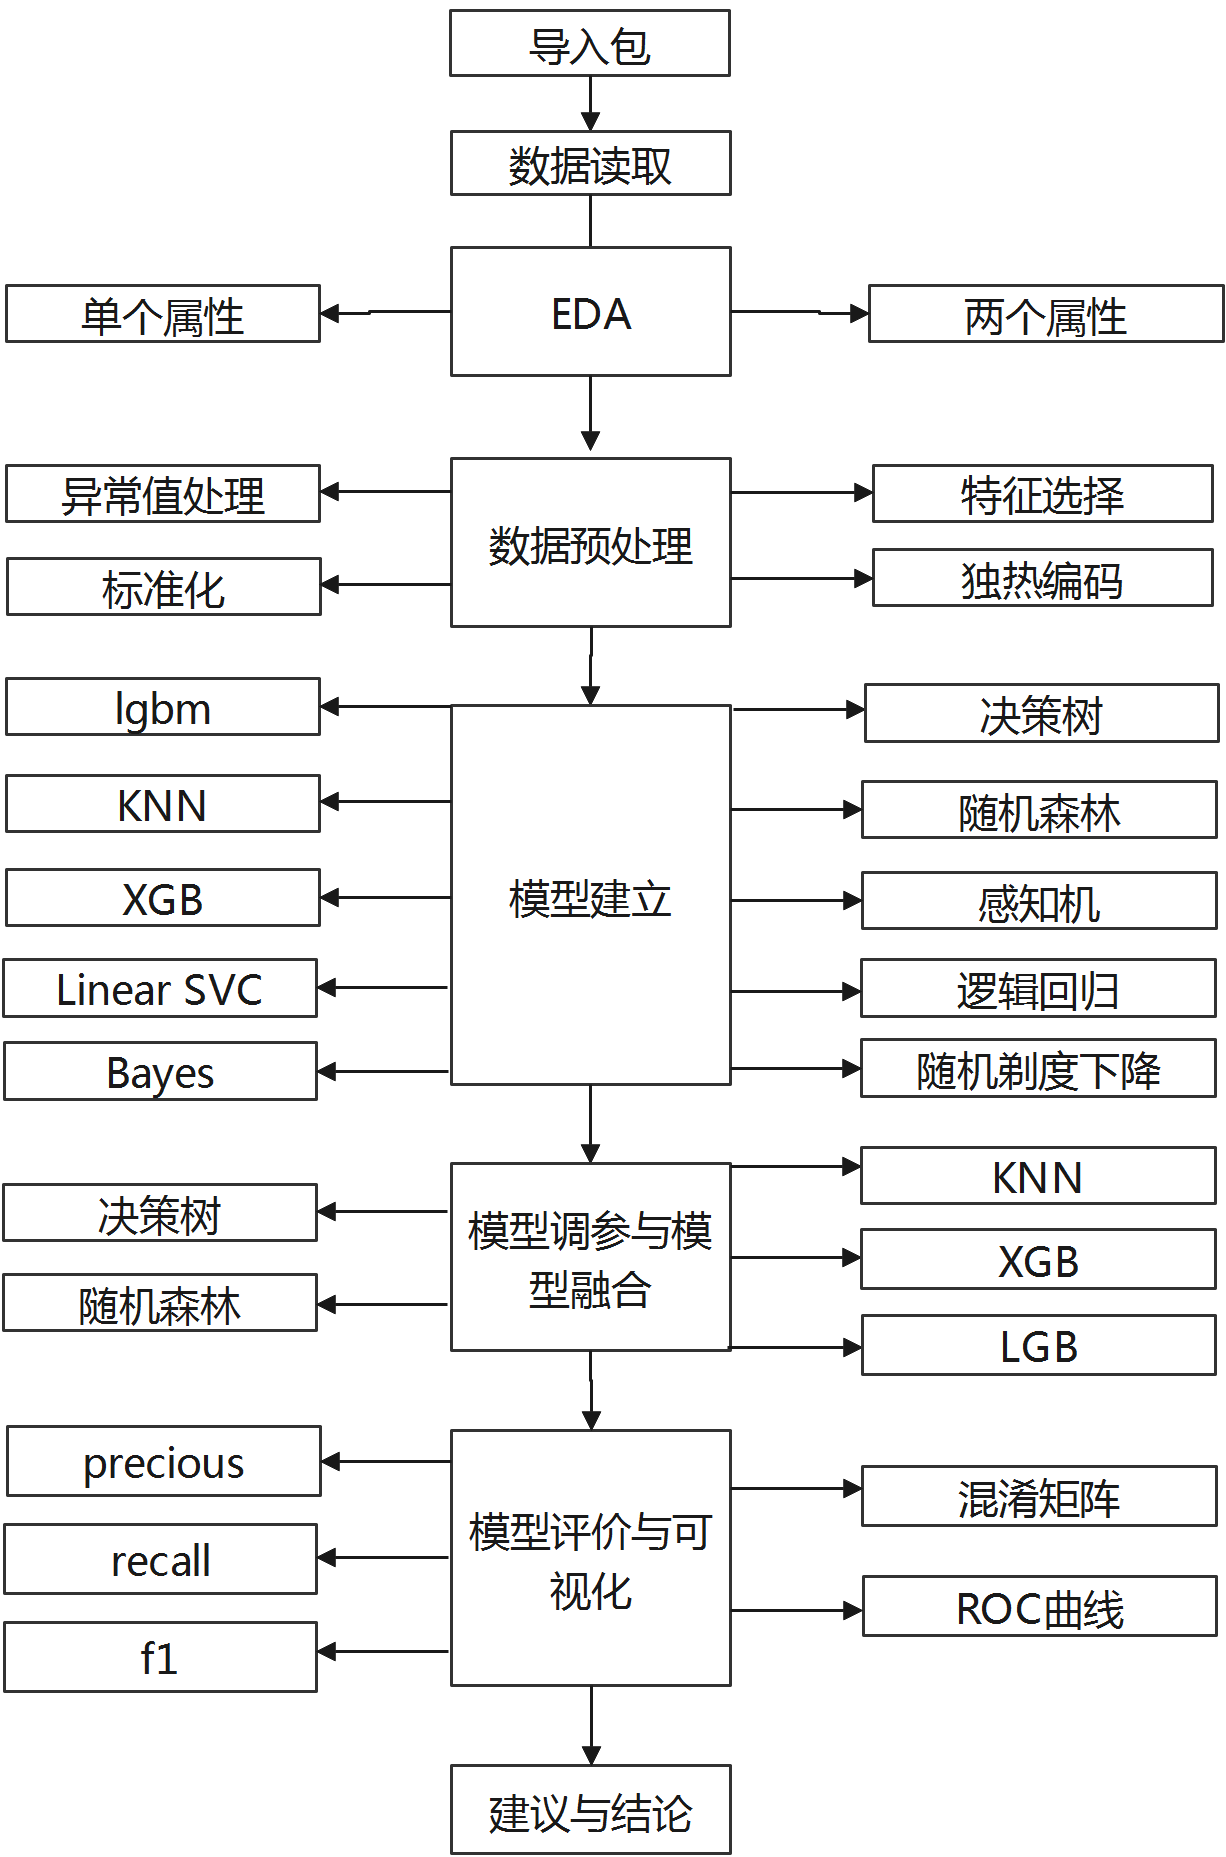
\includegraphics[scale=0.65,angle=0]{images/1.png}
	\caption{论文研究思路}
	\label{1}
\end{figure}


\section{EDA}
\subsection{导入包}
		\begin{figure}[H]
			\centering
			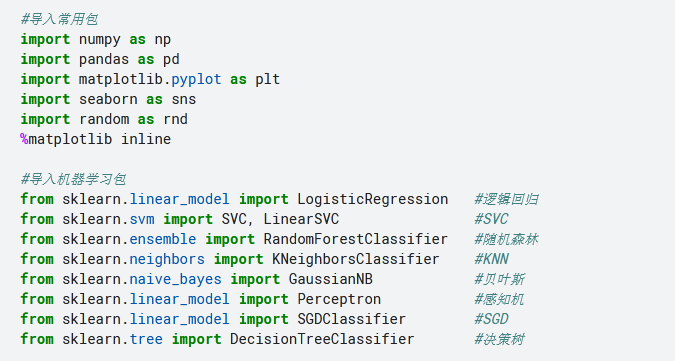
\includegraphics[scale=0.6,angle=0]{images/2.png}
			\caption{导入常用的包}
			\label{2}
		\end{figure}
首先导入需要的包,其中常用包包括了numpy,pandas,matplotlib,seabornscikit-learn的包包括了逻辑回归,SVC,随机森林,KNN,朴素贝叶斯,感知机,SGD和决策树,本文中用于训练并预测信用卡欺诈行为是否发生。

\subsection{数据读取}
\begin{figure}[H]
	\centering
	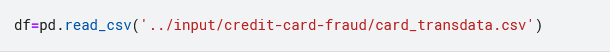
\includegraphics[scale=1.0,angle=0]{images/3.png}
	\caption{读取数据集}
	\label{3}
\end{figure}
使用$pandas$的函数读取数据集,并命名为$df$。
		
\subsection{查看数据基本信息}
通过查看数据行数列数,数据集前五行,基本信息等,获取到以下基本信息:
\begin{itemize}
	\item 没有缺失值;
	\item 数据形状为(1000000,8),包含100万数据、8个属性;
	\item 8个属性之间的相关性接近于0,属性的独立性好,具有优良特征;
	\item 8个属性中$distance\_from\_home$、$distance\_from\_last\_transaction$、$ratio\_to\_median\_purchase\_price$为连续型数据; $repeat\_retailer$、$used\_chip$、$used\_pin\_number$、$online\_order$是取值为0或1的特征;$fraud$是取值为0或1的标签。
\end{itemize}
\begin{figure}[H]
	\centering
	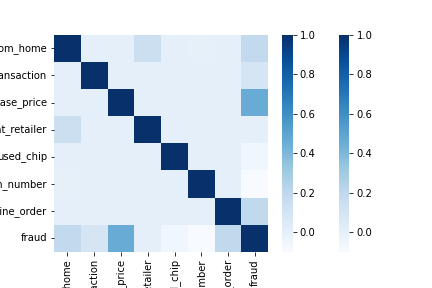
\includegraphics[scale=0.6,angle=0]{images/5.png}
	\caption{属性相关性系数矩阵热力图}
	\label{5}
\end{figure}
\clearpage
\subsection{单个属性数据查看}
绘制7个特征属性的数据分布图如下:
\begin{figure}[H]
	\centering
	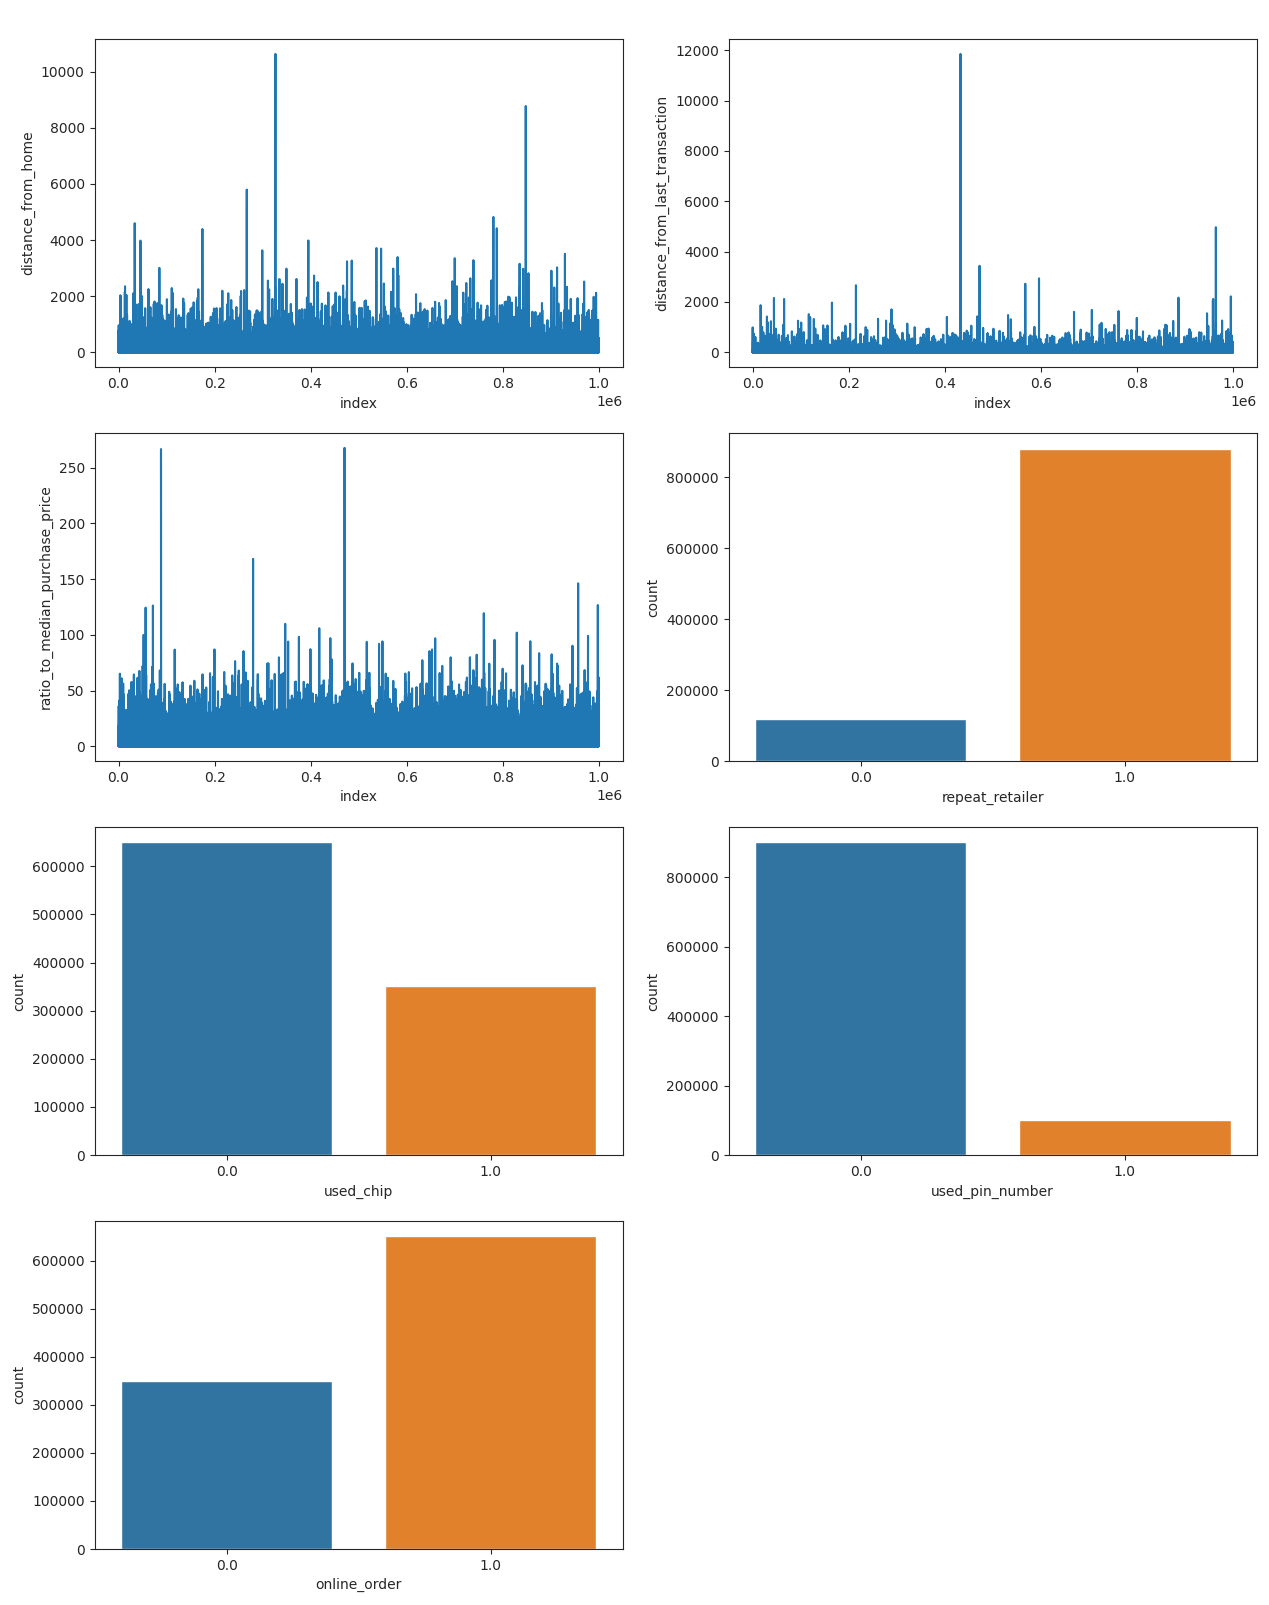
\includegraphics[scale=0.42,angle=0]{images/4.png}
	\caption{数据分布图}
	\label{4}
\end{figure}
通过上图,我们得到以下结论:
\begin{itemize}
	\item $distance\_from\_home$中只有少部分的值超出2000,大部分值在2000以下;
	\item $distance\_from\_last\_transaction$中极少的值超出1000,大部分值在1000以下;
	\item $ratio\_to\_median\_purchase\_price$中只有极少超出100,大部分值在100以下;
	\item 连续型属性只有极少的值发生了严重偏离;推断是出国,境外交易等因素导致;
	\item $repeat\_retailer$图显示,大部分的交易发生在同一个账户;
	\item $used\_chip$图显示,用银行卡交易的订单要比不用银行卡交易的订单多一些;
	\item $used\_pin\_number$图显示,大部分的交易不会使用PIN码进行交易;
	\item $online\_order$图显示,在线交易订单比非在线订单多
\end{itemize}
\subsection{标签关于分类属性的分布}
分别绘制标签在4个分类属性条件下的分布图如下:
\begin{figure}[H]
	\centering
	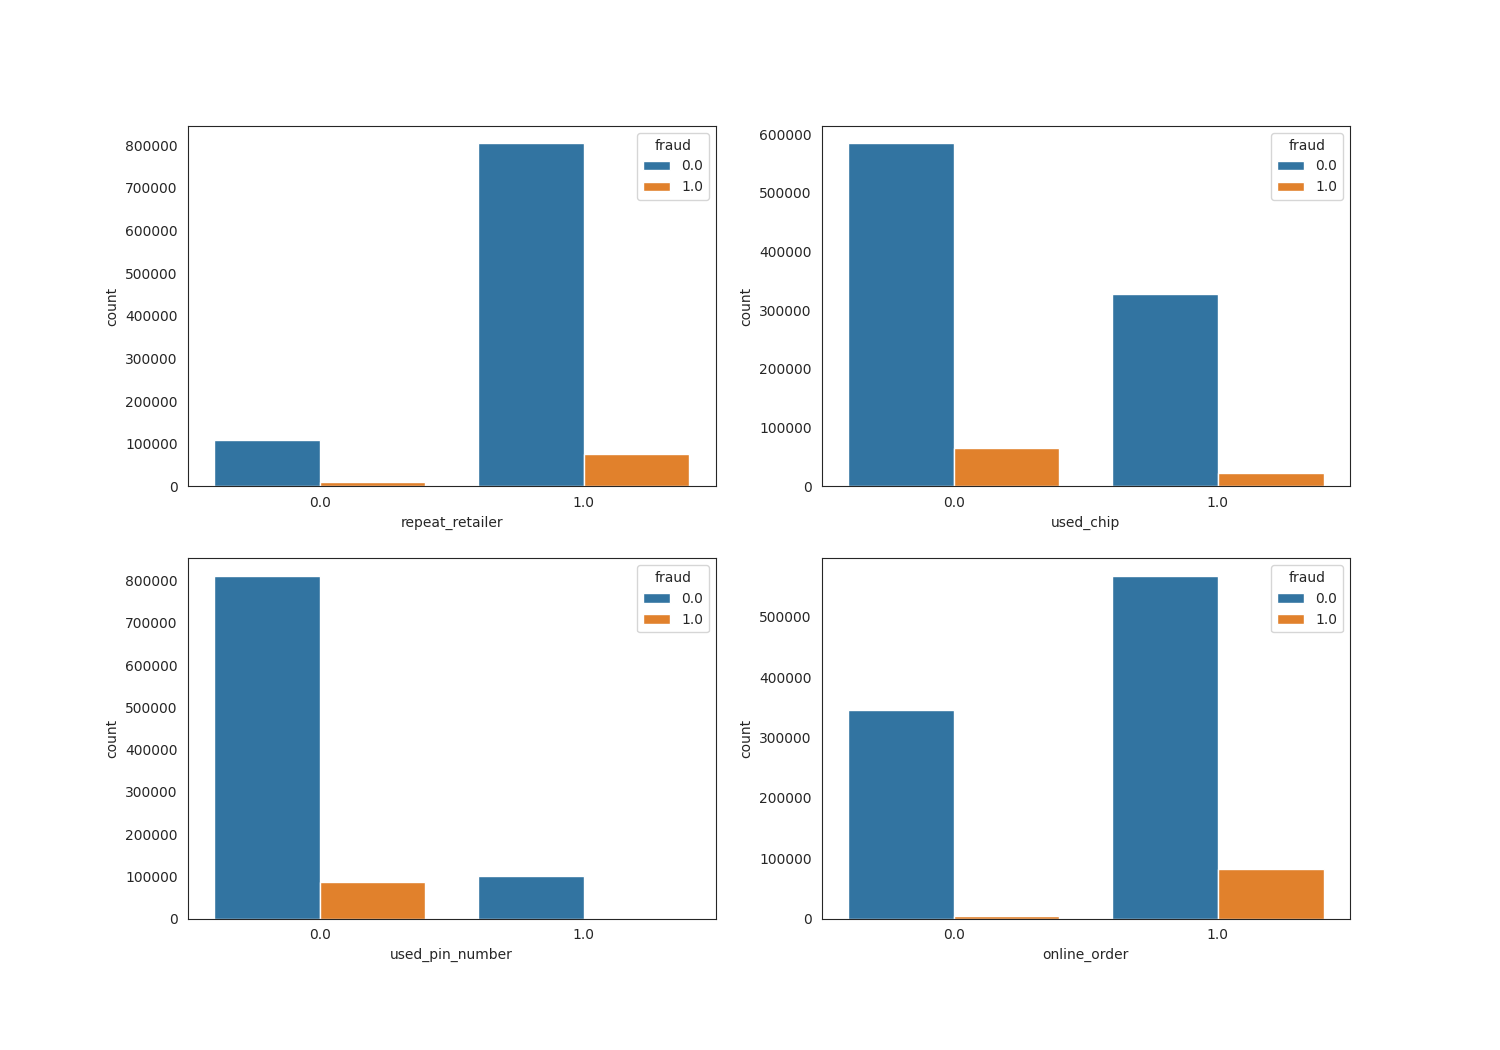
\includegraphics[scale=0.45,angle=0]{images/6.png}
	\caption{标签关于分类属性的分布}
	\label{6}
\end{figure}
\begin{itemize}
	\item $fraud$关于$repeat\_retailer$数据分布图显示,交易发生在同一个账户与不发生在同一个账户发生欺诈行为与不发生欺诈行为的比例相近,也就是说交易发不发生在同一个账户对是否欺诈的影响不大。
	\item $fraud$关于$used\_chip$数据分布图显示,用银行卡交易与不用银行卡交易发生欺诈行为与不发生欺诈行为的比例相近,也就是说是否用银行卡交易对是否欺诈的影响不大。
	\item $used\_pin\_number$图显示,发生欺诈行为的大都是不用pin交易的,用pin交易的没有发生欺诈行为。
	\item $online\_order$图显示,在线交易发生欺诈行为的概率要比非在线交易发生欺诈行为的概率高得多。
\end{itemize}





\section{数据预处理}
	\subsection{异常值处理}
根据前面的分析,3个连续型属性的分布,发现只有极少的值是异常值,考虑到异常数值对应属性在实际生活中是切实存在的,并且异常值处理前后平均值与方差的变化在5\%以内,因此不对数据进行异常值处理。
\subsection{标准化}
对三个连续型属性进行标准化。标准化代码和结果如图:
\begin{figure}[H]
	\centering
	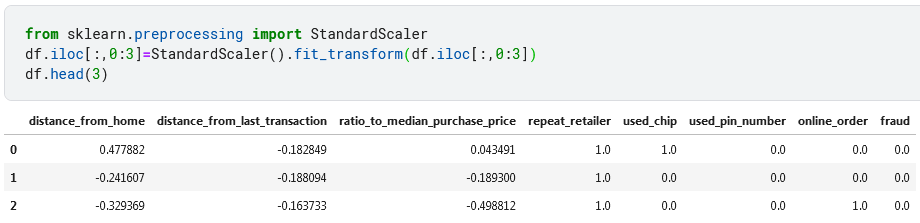
\includegraphics[scale=0.7,angle=0]{images/7.png}
	\caption{标准化}
	\label{7}
\end{figure}

\subsection{独热编码}
对四个分类属性进行独热编码,代码和结果如图:
\begin{figure}[H]
	\centering
	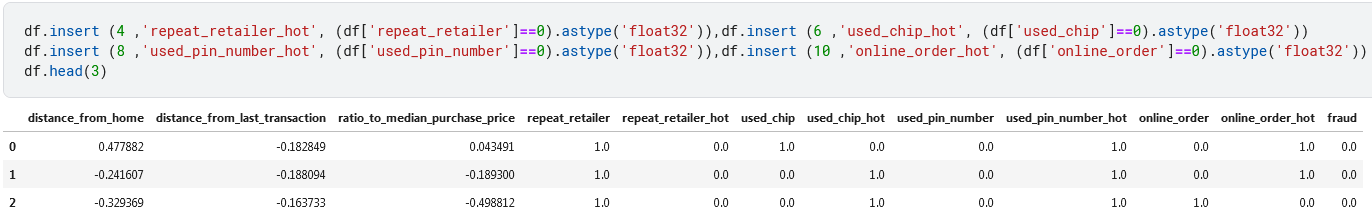
\includegraphics[scale=0.4,angle=0]{images/8.png}
	\caption{独热编码}
	\label{8}
\end{figure}


\subsection{特征选择}
根据图\ref{5}的相关系数矩阵热力图以及相关系数矩阵,发现属性间相关性小,属性独立性好,故没有进一步对数据降维的必要。因此选择所有特征进行分类。


\section{模型建立}
\subsection{数据集划分}
按照训练集:测试集为7:3的比例对数据集进行划分,代码和结果如图:
\begin{figure}[H]
	\centering
	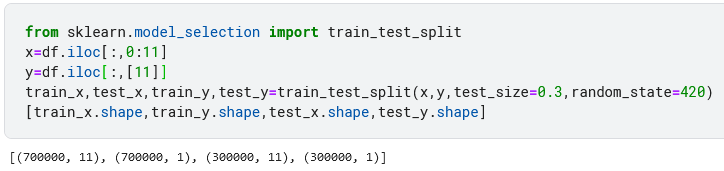
\includegraphics[scale=0.75,angle=0]{images/9.png}
	\caption{数据集划分}
	\label{9}
\end{figure}

\subsection{建立模型并选择调参模型}
使用LGB,XGB,KNN,线性SVC,朴素贝叶斯,决策树,随机森林,感知机,逻辑回归,随机剃度下降10个模型对数据进行拟合并查看在测试集上的准确率如图:
\begin{figure}[H]
	\centering
	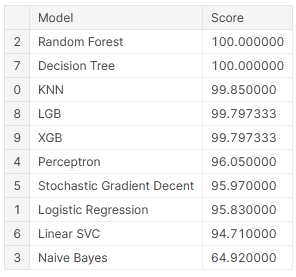
\includegraphics[scale=0.75,angle=0]{images/10.png}
	\caption{模型得分}
	\label{10}
\end{figure}
其中决策树,随机森林的准确率达到了\textbf{100\%},LGB,XGB,KNN均有较高的准确率。


\section{模型调参与模型融合}
\subsection{模型调参}
选用LGB,XGB,KNN,决策树,随机森林评分最高的5个模型进行调参,使用5折交叉验证,使用网格搜索对参数进行优化,其中随机森林的调参代码和结果如下:
\begin{figure}[H]
	\centering
	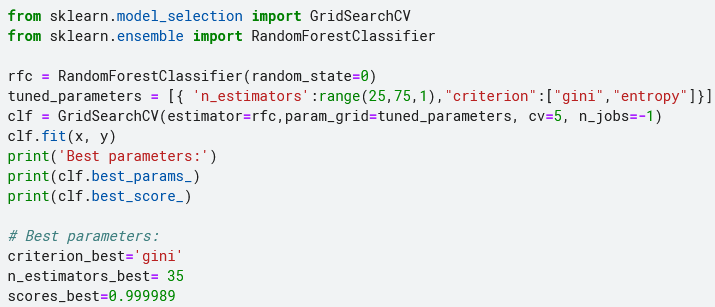
\includegraphics[scale=0.75,angle=0]{images/11.png}
	\caption{调参代码}
	\label{11}
\end{figure}
选取得分最高的参数作为最终模型,参数调节前后模型的变化如下图:
\begin{figure}[H]
	\centering
	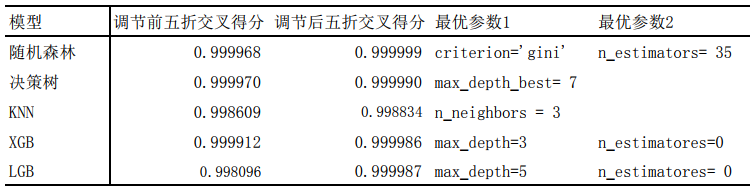
\includegraphics[scale=0.75,angle=0]{images/12.png}
	\caption{调参结果}
	\label{12}
\end{figure}


\subsection{模型融合}
选取调参后表现最高的LGB,XGB,随机森林搭建Stacking模型,代码如下:
\begin{figure}[H]
	\centering
	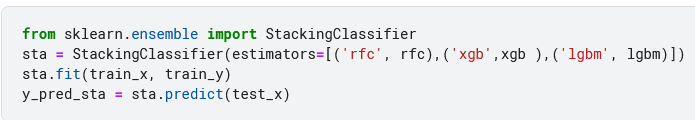
\includegraphics[scale=0.6,angle=0]{images/13.png}
	\caption{Stacking模型}
	\label{13}
\end{figure}

\section{模型评价与可视化}
根据上面的6个模型,求出模型5折交叉验证准确率,precious,recall,F-1分数值如下:
\begin{figure}[H]
	\centering
	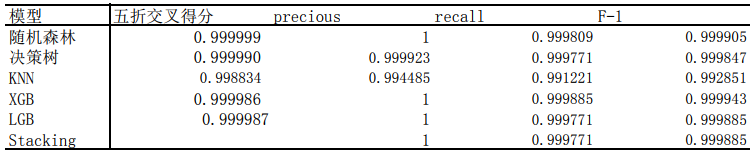
\includegraphics[scale=0.57,angle=0]{images/15.png}
	\caption{模型评价指标}
	\label{15}
\end{figure}
分别绘制6个模型在测试集上的混淆矩阵如图:
\begin{figure}[H]
	\centering
	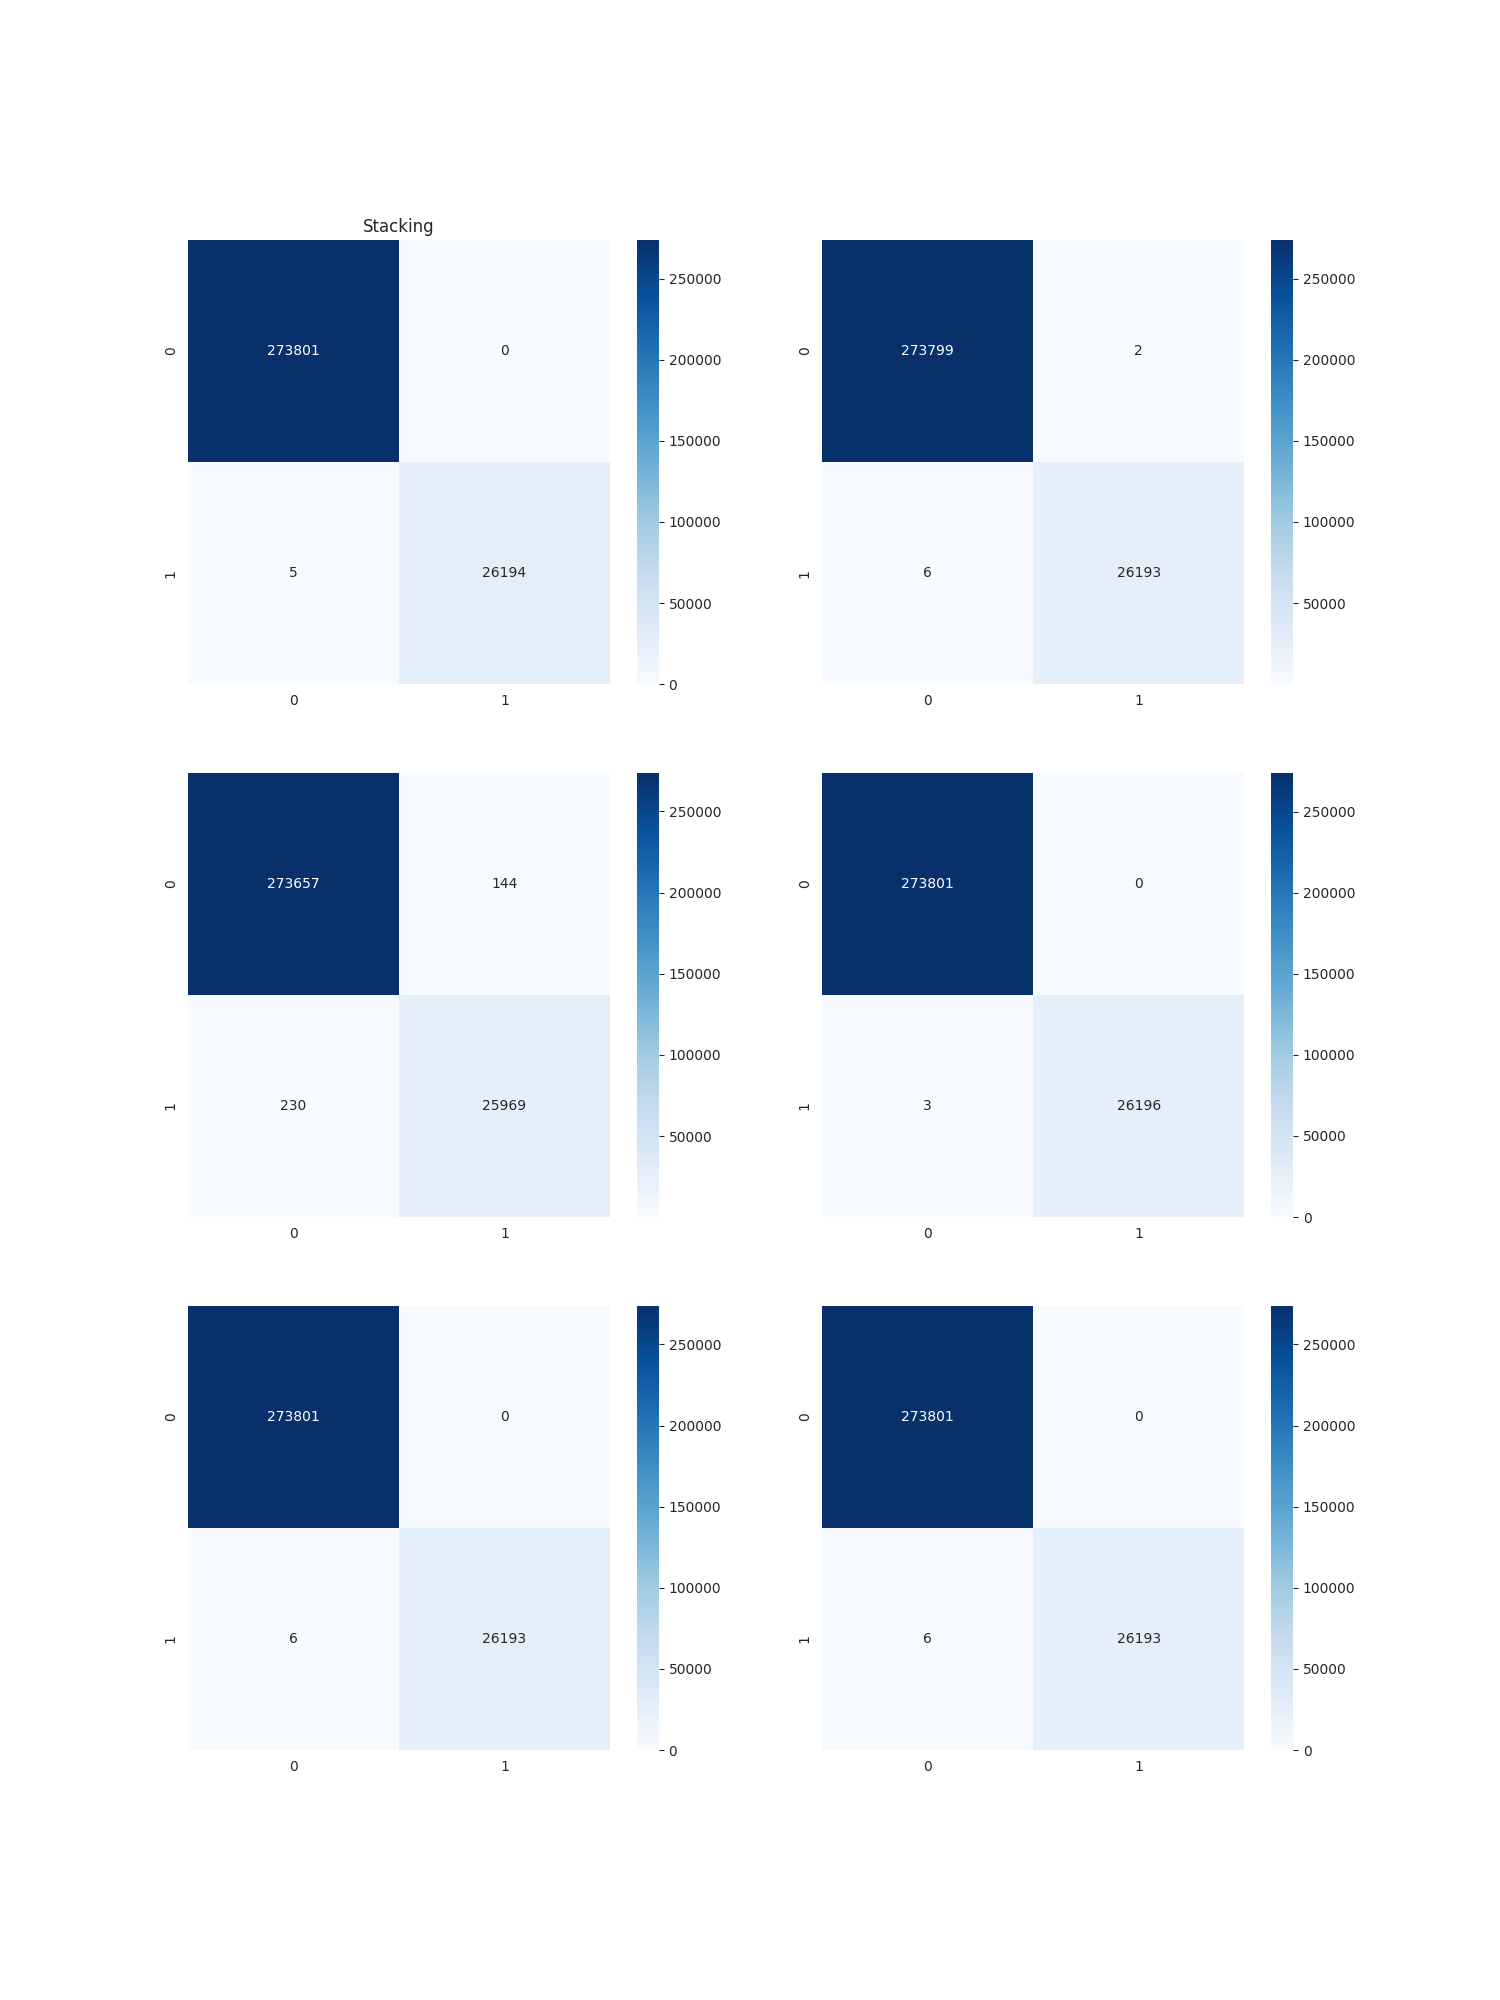
\includegraphics[scale=0.3,angle=0]{images/16.png}
	\caption{混淆矩阵}
	\label{16}
\end{figure}


通过绘制6个图的ROC曲线发现,LGB,XGB,KNN,决策树,随机森林,Stacking的模型的ROC曲线均相和下图相同:
\begin{figure}[H]
	\centering
	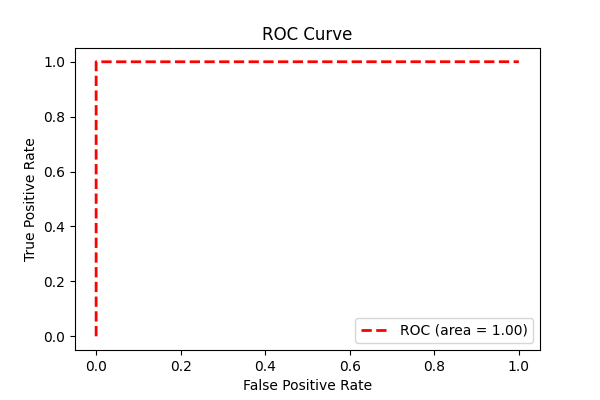
\includegraphics[scale=0.75,angle=0]{images/17.png}
	\caption{ROC曲线}
	\label{17}
\end{figure}
从以上的模型可以看出,模型之间的差别已经不大,根据五折交叉得分和F1分数值最终选择Stackin作为最终模型,模型准确率为0.9999987,F-1值为0.999885。


\section{建议与结论}
\subsection{建议}
根据fraud与各个属性的相关性系数以及结合本文EDA部分的结论,我们提出一下建议:用户如果能够使用pin交易,那么将会使欺诈发生的概率趋近于0;当用户发现当前交易是往期交易的数倍时,用户需要谨慎思考当前是否遭遇了银行卡欺诈行为。

\subsection{结论}
最终选择Stackin作为最终模型,模型准确率为0.9999987,F-1值为0.999885。








\begin{thebibliography}{99}
	\bibitem{book2}周志华. 机器学习 [J]. 清华大学出版社, 2016, 8(28): 1–415.
\end{thebibliography}	


	


%\include{sections/Experimentalmaterials}
%\include{sections/Micro-organizationanalysis}
%\include{sections/Mechanicsperformanceanalysis}

%\include{sections/conclusion}
%\include{sections/thanks}

%\bibliographystyle{plain}
\bibliographystyle{unsrt}
\nocite{*}
\addcontentsline{toc}{section*}{参考文献}

\renewcommand\bibnumfmt[1]{\makebox[0.9cm][l]{[#1]}}
\setlength{\bibhang}{0em}


%\begin{thebibliography}{99}
%	\bibitem{book1}邓集贤,杨维权,司徒荣,邓永录.概率论与数理统计.下册(第四版).北京:高等教育出版社,2009.7
%\end{thebibliography}	




%\include{sections/appendix}

\end{document}